%%%%%%%%%%%%%%%%%%%%%%%%%%%%%%%%%%%%%%%%%%%%%%%%%%%%%%%%%%%%%%%%%%%%%%%%%%%%%%%%
%                                                                              %
%                              Required Packages                               %
%                                                                              %
%%%%%%%%%%%%%%%%%%%%%%%%%%%%%%%%%%%%%%%%%%%%%%%%%%%%%%%%%%%%%%%%%%%%%%%%%%%%%%%%

% Basic packages.
\usepackage[utf8]{inputenc}
\usepackage[T1]{fontenc}
% Gives us multiple colors.
\usepackage[usenames,dvipsnames,pdftex]{xcolor}
% Lets us style link colors.
\usepackage{hyperref,theoremref}
% Lets us import images and graphics.
\usepackage{graphicx}
% Let's us modify list stuff.
\usepackage{enumitem}
% Lets us use figures in floating environments.
\usepackage{float}
% Lets us create multiple columns.
\usepackage{multicol}
\usepackage{multirow}
\usepackage{array}
% Gives us better math syntax.
\usepackage{amsmath,amsfonts,mathtools,amsthm,amssymb}
% Lets us strike through text.
\usepackage{cancel}
% Lets us import pdf directly in our tex code.
\usepackage{pdfpages}
% Derivative stuff.
\usepackage{derivative}
% Table stuff.
\usepackage{tablists}
\usepackage{tabularx}
\usepackage{wasysym}
\usepackage{booktabs}
\usepackage{subcaption}
\usepackage{dcolumn}
% Lets us get the title, author, and date.
\usepackage{authoraftertitle}
% Set the geometry.
\usepackage[tmargin=2cm,rmargin=1in,lmargin=1in,margin=0.85in,bmargin=2cm,footskip=1cm]{geometry}
% Useful for creating mini table of contents.
\usepackage{minitoc}
% Useful for referencing.
\usepackage[noabbrev]{cleveref}
% Other.
\usepackage{nameref}
\usepackage{anyfontsize}
\usepackage{sectsty}
\usepackage{soul}
\usepackage{empheq}


%%%%%%%%%%%%%%%%%%%%%%%%%%%%%%%%%%%%%%%%%%%%%%%%%%%%%%%%%%%%%%%%%%%%%%%%%%%%%%%%
%                                                                              %
%                                Basic Settings                                %
%                                                                              %
%%%%%%%%%%%%%%%%%%%%%%%%%%%%%%%%%%%%%%%%%%%%%%%%%%%%%%%%%%%%%%%%%%%%%%%%%%%%%%%%

%%%%%%%%%
% Tasks %
%%%%%%%%%

\usepackage{tasks}
\usepackage{extramarks}

\settasks{label=\bfseries\arabic*.),label-width=2em}

%%%%%%%%%%%
%  Table  %
%%%%%%%%%%%

\newcolumntype{C}{>{\Centering\arraybackslash}X}
\setlength{\tabcolsep}{5pt}
\renewcommand\arraystretch{1.5}

% Caption setup.
\usepackage[font=bf]{caption}
\renewcommand\thetable{\Roman{table}}
\captionsetup[figure]{font=small}
\captionsetup{justification=centering}

%%%%%%%%%%%%%
%  Symbols  %
%%%%%%%%%%%%%

\allowdisplaybreaks
\let\implies\Rightarrow
\let\impliedby\Leftarrow
\let\iff\Leftrightarrow
\let\epsilon\varepsilon
\let\svlim\lim\def\lim{\svlim\limits}
\let\svsum\sum\def\sum{\svsum\limits}

%%%%%%%%%%%
%  Lists  %
%%%%%%%%%%%

\setlist[itemize,1]{label=--}
\setlist[itemize,2]{label=\textbullet}
\setlist[enumerate,1]{label=\protect\circled{\arabic*}}

%%%%%%%%%%%%%%
%  SI Unitx  %
%%%%%%%%%%%%%%

\usepackage{siunitx}
\sisetup{
  locale = US,
  per-mode = symbol,
  propagate-math-font = true,
  reset-math-version = false,
  exponent-mode = engineering,
  round-mode = figures,
  round-precision = 3,
  drop-zero-decimal,
}

% Distance
\DeclareSIUnit{\millimeter}{mm}
\DeclareSIUnit{\centimeter}{cm}
\DeclareSIUnit{\decimeter}{dm}
\DeclareSIUnit{\inch}{in}
\DeclareSIUnit{\foot}{ft}
\DeclareSIUnit{\yard}{yd}
\DeclareSIUnit{\meter}{m}
\DeclareSIUnit{\kilometer}{km}
\DeclareSIUnit{\mile}{mi}
\DeclareSIUnit{\astronomicalunit}{au}
\DeclareSIUnit{\lightyear}{ly}

% Temperature
\DeclareSIUnit{\fahrenheit}{F}
\DeclareSIUnit{\celsius}{C}

% Time
\DeclareSIUnit{\millisecond}{ms}
\DeclareSIUnit{\second}{sec}
\DeclareSIUnit{\minute}{min}
\DeclareSIUnit{\hour}{hr}
\DeclareSIUnit{\day}{d}
\DeclareSIUnit{\week}{wk}
\DeclareSIUnit{\month}{mos}
\DeclareSIUnit{\year}{yr}

% Weight
\DeclareSIUnit{\milligram}{mg}
\DeclareSIUnit{\gram}{g}
\DeclareSIUnit{\ounce}{oz}
\DeclareSIUnit{\pound}{lb}
\DeclareSIUnit{\kilogram}{kg}
\DeclareSIUnit{\ton}{t}

% Liquid
\DeclareSIUnit{\gallon}{gal}
\DeclareSIUnit{\liter}{L}
\DeclareSIUnit{\milliliter}{mL}

%%%%%%%%%%
%  TikZ  %
%%%%%%%%%%

\usepackage[framemethod=TikZ]{mdframed}
\usepackage{tikz}
\usepackage{tkz-euclide}
\usepackage{tikz-cd}
\usepackage{animate}
\usepackage{bm}

\usetikzlibrary{
  intersections,
  angles,
  quotes,
  calc,
  positioning,
  3d,
  arrows,
  arrows.meta,
  patterns,
}

\tikzset{>=stealth}

%%%%%%%%%%%%%%%
%  PGF Plots  %
%%%%%%%%%%%%%%%

\usepackage{pgfplots}
\usepackage{pgfplotstable}

\pgfplotsset{compat=1.18}

\usepgfplotslibrary{fillbetween}
\usepgfplotslibrary{patchplots}
\usepgfplotslibrary{external}
\usetikzlibrary{decorations.pathreplacing,calligraphy}
\tikzexternalenable

\definecolor{linecolor1}{HTML}{3DC6F3}
\definecolor{linecolor2}{HTML}{F034A3}
\definecolor{linecolor3}{HTML}{F57215}
\definecolor{linecolor4}{HTML}{733786}
\definecolor{linecolor5}{HTML}{80CF5C}

\pgfplotsset{style1/.style={color=linecolor1,mark=none,line width=1pt,solid}}
\pgfplotsset{style2/.style={color=linecolor2,mark=none,line width=1pt,solid}}
\pgfplotsset{style3/.style={color=linecolor3,mark=none,line width=1pt,solid}}
\pgfplotsset{style4/.style={color=linecolor4,mark=none,line width=1pt,solid}}
\pgfplotsset{style5/.style={color=linecolor5,mark=none,line width=1pt,solid}}
\pgfplotsset{asymptote/.style={color=gray,mark=none,line width=1pt,<->,dashed}}
\pgfplotsset{soldot/.style={color=linecolor2,only marks,mark=*}}
\pgfplotsset{holdot/.style={color=linecolor2,fill=white,only marks,mark=*}}
\pgfplotsset{integration/.style={name path=curve,color=linecolor1,mark=none,line width=0.5pt,solid}}

\pgfplotscreateplotcyclelist{pccstylelist}{
  style1,
  style2,
  style3,
  style4,
  style5,
}

\def\axisdefaultwidth{175pt}
\def\axisdefaultheight{\axisdefaultwidth}
\pgfplotsset{
  every axis/.append style={
    axis x line=middle, x axis line style={name path=xaxis},
    axis y line=middle, y axis line style={name path=yaxis},
    ticks=none,
    axis line style={->},
    xlabel={$x$},
    ylabel={$y$},
    samples=1000,
    cycle list name=pccstylelist
  },
}

%%%%%%%%%%%%%%%%%%%%%%%
%  Center Title Page  %
%%%%%%%%%%%%%%%%%%%%%%%

\usepackage{titling}
\renewcommand\maketitlehooka{\null\mbox{}\vfill}
\renewcommand\maketitlehookd{\vfill\null}

%%%%%%%%%%%%%%%%%%%%%%%%%%%%%%%%%%%%%%%%%%%%%%%%%%%%%%%
%  Create a grey background in the middle of the PDF  %
%%%%%%%%%%%%%%%%%%%%%%%%%%%%%%%%%%%%%%%%%%%%%%%%%%%%%%%

\usepackage{eso-pic}

\newcommand\definegraybackground{
  \definecolor{reallylightgray}{HTML}{FAFAFA}
  \AddToShipoutPicture{
    \ifthenelse{\isodd{\thepage}}{
      \AtPageLowerLeft{
        \put(\LenToUnit{\dimexpr\paperwidth-222pt},0){
          \color{reallylightgray}\rule{222pt}{297mm}
        }
      }
    }
    {
      \AtPageLowerLeft{
        \color{reallylightgray}\rule{222pt}{297mm}
      }
    }
  }
}

%%%%%%%%%%%%%%%%%%%
%  Footnote Line  %
%%%%%%%%%%%%%%%%%%%

\renewcommand\footnoterule{\hrule\vspace{0.1cm}}

%%%%%%%%%%%%%%%%%%%%%%%%
%  Modify Links Color  %
%%%%%%%%%%%%%%%%%%%%%%%%

\hypersetup{
  colorlinks,
  linkcolor=main!90,
  citecolor=black,
  urlcolor=black,
}

%%%%%%%%%%%%%%%%%%
% Fix WrapFigure %
%%%%%%%%%%%%%%%%%%

\newcommand{\wrapfill}{\par\ifnum\value{WF@wrappedlines}>0
  \parskip=0pt
  \addtocounter{WF@wrappedlines}{-1}%
  \null\vspace{\arabic{WF@wrappedlines}\baselineskip}%
  \WFclear
\fi}

%%%%%%%%%%%%%%%%%
% Multi Columns %
%%%%%%%%%%%%%%%%%

\let\multicolmulticols\multicols
\let\endmulticolmulticols\endmulticols

\RenewDocumentEnvironment{multicols}{mO{}}
{%
  \ifnum#1=1
    #2%
  \else
    \multicolmulticols{#1}[#2]
  \fi
}
{%
  \ifnum#1=1
  \else
    \endmulticolmulticols
  \fi
}

\newlength{\thickarrayrulewidth}
\setlength{\thickarrayrulewidth}{5\arrayrulewidth}


%%%%%%%%%%%%%%%%%%%%%%%%%%%%%%%%%%%%%%%%%%%%%%%%%%%%%%%%%%%%%%%%%%%%%%%%%%%%%%%%
%                                                                              %
%                           School Specific Commands                           %
%                                                                              %
%%%%%%%%%%%%%%%%%%%%%%%%%%%%%%%%%%%%%%%%%%%%%%%%%%%%%%%%%%%%%%%%%%%%%%%%%%%%%%%%

%%%%%%%%%%%%%%%%%%%%%%
%  Helpful Commands  %
%%%%%%%%%%%%%%%%%%%%%%

\makeatletter

\newcommand\resetcounters{
  \setcounter{section}{0}
  \setcounter{subsection}{0}
  \setcounter{subsubsection}{0}
  \setcounter{paragraph}{0}
  \setcounter{subparagraph}{0}
}

%%%%%%%%%%%%%%%%%%%%%%%%%%%%%
%  Lecture/Chapter Command  %
%%%%%%%%%%%%%%%%%%%%%%%%%%%%%

\usepackage{ifthen}
\usepackage{xifthen}

\def\@notenum{}
\newcommand\includenote[1]{
  \ifnum #1<10
    \def\@notenum{0#1}
  \else
    \def\@notenum{#1}
  \fi

  % Set the chapter counter to the number passed.
  \setcounter{chapter}{#1}
  % Reset all counters.
  \resetcounters
  % Include the note file if it exists.
  \IfFileExists{\noteloc-\@notenum.tex}{\input{\noteloc-\@notenum.tex}}{}
}

\newcommand{\localtoc}{
  \startcontents
  \printcontents{}{1}{\noindent{\color{main}\rule{\textwidth}{0.4pt}\par}\vspace*{-0.3cm}\subsection*{{\color{main}Lecture Note Overview}}}
  \noindent{{\color{main}\rule{\textwidth}{0.4pt}\par}}
}

\def\@note{}
\def\@notetbl{}
\NewDocumentCommand\nte{O{} O{} m m}{%
  \ifthenelse{\isempty{#3}}{%
    \def\@note{\lecorchap~\arabic{chapter}}
  }{%
    \def\@note{\lecorchap~\arabic{chapter}: #4}
  }%
  \def\@notetbl{\lecorchap~\arabic{chapter}}
  {\fontsize{10}{12}\selectfont\sffamily\ifstrequal{#1}{}{}{\noindent#1}\ifstrequal{#3}{}{}{\hfill#3}}
  \vspace*{0.03cm}
  \hrule
  \vspace*{-0.3cm}
  \phantomsection\addcontentsline{toc}{chapter}{\protect\numberline{\thechapter}#4}
  \section*{{\fontsize{20}{30}\selectfont\@note}}
  \ifstrequal{#2}{false}{}{\localtoc}
}

%%%%%%%%%%%%%%%%%
% Fancy Headers %
%%%%%%%%%%%%%%%%%

\usepackage{fancyhdr}

\newcommand\createintro{
  % Create title page.
  \mytitle
  % Force newpage.
  \clearpage\mbox{~}\clearpage\newpage

  % Create the introduction header on the intro page.
  \pagenumbering{roman}
  \begin{center}
    \textbf{{\LARGE Introduction}}
  \end{center}

  % Check if the intro.tex file exists.
  % If it does, include it, otherwise, just ignore.
  \IfFileExists{./intro.tex}{{\small
  \noindent\textbf{Topic One}\\
  Brief explanation.\hspace*{\fill}

  \vspace{10pt}
  \noindent\textbf{Topic Two}\\
  Brief explanation.\hspace*{\fill}
}
}{}

  % Set the pagestyle to fancy.
  \pagestyle{fancy}
  % Remove the header line.
  \renewcommand\headrulewidth{0pt}

  % Reset fancyhead styles.
  \fancyhead{}
  % Add a fancyfoot center style.
  \fancyfoot[C]{%
    \textit{For more notes like this, visit \href{\linktootherpages}{\shortlinkname}}.%
  }%

  % Create a box with more information.
  \vspace{0.5cm}
  \begin{tcolorbox}[enhanced,colback=white,center upper,size=fbox, drop shadow southwest,sharp corners]
    \term: \academicyear, \\
    Last Update: \today, \\
    \faculty, \location.
  \end{tcolorbox}

  % Create a new page.
  \newpage
  % Display table of contents.
  \tableofcontents

  % Change the numbering style back to arabic from roman.
  \pagenumbering{arabic}
  % Reset page numbers back to 1.
  \setcounter{page}{1}

  % Add back the header line.
  \renewcommand\headrulewidth{0.4pt}
  % Add the lecture/chapter name in the top right.
  \fancyhead[R]{\@note}
  % Add the author name in the top left.
  \fancyhead[L]{\@author}
  % Add the page number in the bottom center.
  \fancyfoot[C]{\thepage}
  \@ifclasswith\class{grayfg}{%
    % If user passed grayfg as a parameter to \documentclass, then set the rest
    % of the page to two column.
    \definegraybackground%
  }{}
}

%%%%%%%%%%%%%%%%%%%%
%  Import Figures  %
%%%%%%%%%%%%%%%%%%%%

\usepackage{import}
\pdfminorversion=7
\newcommand\incfig[2][1]{
  \def\svgwidth{#1\columnwidth}
  \import{\figloc-\@notenum}{#2.pdf_tex}
}

%%%%%%%%%%%%
%  Circle  %
%%%%%%%%%%%%

\newcommand*\circled[1]{\tikz[baseline=(char.base)]{
  \node[shape=circle,draw,inner sep=1pt] (char) {#1};}
}

%%%%%%%%%%%%%
%  Correct  %
%%%%%%%%%%%%%

\definecolor{correct}{HTML}{009900}
\newcommand\correct[2]{{\color{red}{#1 }}\ensuremath{\to}{\color{correct}{ #2}}}

%%%%%%%%%%%%%%%
%  Important  %
%%%%%%%%%%%%%%%

\newcommand\imp[1]{{\color{main}#1}}

%%%%%%%%%
%  QED  %
%%%%%%%%%

\usepackage{stmaryrd}
\newcommand\contra{\phantom\hfill\scalebox{1.1}{$\lightning$}}

%%%%%%%%%%%%%%%%%%%
%  Todo Commands  %
%%%%%%%%%%%%%%%%%%%

\usepackage[colorinlistoftodos]{todonotes}

\makeatletter

\@ifclasswith\class{working}{
  \newcommand\improvement[2][]{\todo[linecolor=Plum,backgroundcolor=Plum!25,bordercolor=Plum,#1]{#2}}
  \newcommand\unsure[2][]{\todo[linecolor=red,backgroundcolor=red!25,bordercolor=red,#1]{#2}}
  \newcommand\change[2][]{\todo[linecolor=yellow,backgroundcolor=yellow!25,bordercolor=yellow,#1]{#2}}
  \newcommand\add[2][]{\todo[linecolor=blue,backgroundcolor=blue!25,bordercolor=blue,#1]{#2}}
  \newcommand\info[2][]{\todo[linecolor=OliveGreen,backgroundcolor=OliveGreen!25,bordercolor=OliveGreen,#1]{#2}}

  \newcommand\improvementinline[2][]{\todo[inline,linecolor=Plum,backgroundcolor=Plum!25,bordercolor=Plum,#1]{#2}}
  \newcommand\unsureinline[2][]{\todo[inline,linecolor=red,backgroundcolor=red!25,bordercolor=red,#1]{#2}}
  \newcommand\changeinline[2][]{\todo[inline,linecolor=yellow,backgroundcolor=yellow!25,bordercolor=yellow,#1]{#2}}
  \newcommand\addinline[2][]{\todo[inline,linecolor=blue,backgroundcolor=blue!25,bordercolor=blue,#1]{#2}}
  \newcommand\infoinline[2][]{\todo[inline,linecolor=OliveGreen,backgroundcolor=OliveGreen!25,bordercolor=OliveGreen,#1]{#2}}
  \newcommand\listnotes{
    \newpage
    \listoftodos[Notes]
  }
}{
  \newcommand\improvement[2][]{}
  \newcommand\unsure[2][]{}
  \newcommand\change[2][]{}
  \newcommand\add[2][]{}
  \newcommand\info[2][]{}

  \newcommand\improvementinline[2][]{}
  \newcommand\unsureinline[2][]{}
  \newcommand\changeinline[2][]{}
  \newcommand\addinline[2][]{}
  \newcommand\infoinline[2][]{}
  \newcommand\listnotes{}
}

\makeatother

%%%%%%%%%%%%%%%%%%%%%%%%%%%%%%%%%%%%%%%%%%%%%%
%  Edit Sections/Subsections/Subsubsections  %
%%%%%%%%%%%%%%%%%%%%%%%%%%%%%%%%%%%%%%%%%%%%%%

\usepackage{titlesec}

\makeatletter
\titleformat*{\section}{\sffamily\fontsize{14}{16}\bfseries}
\titleformat*{\subsection}{\sffamily\fontsize{12}{14}\bfseries}
\titleformat{\subsubsection}{\color{subsubsection}\sffamily\fontsize{11}{14}\bfseries}{}{0em}{}
\def\@seccntformat#1{\llap{\csname the#1\endcsname\quad}}
\makeatother

%%%%%%%%%%%%%%%%%%%%%%%%%%%%%%%%%%
%  Edit equation number display  %
%%%%%%%%%%%%%%%%%%%%%%%%%%%%%%%%%%

\makeatletter
\renewcommand\theequation{\arabic{equation}}
\renewcommand\tagform@[1]{%
  {\color{main}\boxed{\textbf{#1}}}
}
\def\@eqnnum{{\normalfont \normalcolor \theequation}}
\makeatother

%%%%%%%%%%%%%%%%%%
%  Equivalently  %
%%%%%%%%%%%%%%%%%%

\newcommand\equivalently[1]{[ \textbf{Equivalently:} #1 ]}

%%%%%%%%%%%%%%%%%%%%%
%  L'Hopital's Rule %
%%%%%%%%%%%%%%%%%%%%%

\newcommand\lop{\stackrel{\textrm{H}}{=}}

%%%%%%%%%%%%%%%%
%  Check mark  %
%%%%%%%%%%%%%%%%

\def\checkmark{\tikz\fill[scale=0.4](0,.35) -- (.25,0) -- (1,.7) -- (.25,.15) -- cycle;} 

%%%%%%%%%%%%%%
%  Vinculum  %
%%%%%%%%%%%%%%

\newcommand\vinculum[1]{\frac{\hspace{#1cm}}{}}

%%%%%%%%%%%%%%%%%%%
%  Wrong Concept  %
%%%%%%%%%%%%%%%%%%%

\newcommand{\wconc}{%
  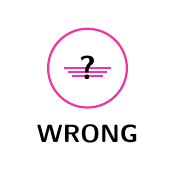
\begin{tikzpicture}[baseline=-0.5ex, scale=0.1]
    \draw[main, thick] circle (5);
    \draw[main, thick] (-3,0) -- (3,0);
    \draw[main, thick] (-2.5,-0.5) -- (2.5,-0.5);
    \draw[main, thick] (-2,-1) -- (2,-1);
    \node[font=\sffamily\bfseries\large] at (0,0) {?};
    \node[font=\sffamily\bfseries\small, anchor=north] at (0,-6) {WRONG};
  \end{tikzpicture}%
}


%%%%%%%%%%%%%%%%%%%%%%%%%%%%%%%%%%%%%%%%%%%%%%%%%%%%%%%%%%%%%%%%%%%%%%%%%%%%%%%%
%                                                                              %
%                                 Environments                                 %
%                                                                              %
%%%%%%%%%%%%%%%%%%%%%%%%%%%%%%%%%%%%%%%%%%%%%%%%%%%%%%%%%%%%%%%%%%%%%%%%%%%%%%%%

\usepackage{varwidth}
\usepackage{thmtools}
\usepackage{etoolbox}
\usepackage[most,many,breakable]{tcolorbox}

\mdfsetup{skipabove=1em,skipbelow=0em}
\tcbuselibrary{theorems,skins,hooks}

%%%%%%%%%%%%%%%%%%%
%  Define Colors  %
%%%%%%%%%%%%%%%%%%%

\makeatletter

\definecolor{main}{HTML}{F035A3}
\definecolor{solution}{HTML}{00AEEF}
\definecolor{qedsolution}{HTML}{76B4CF}
\definecolor{proof}{HTML}{F035A3}
\definecolor{subsubsection}{HTML}{B00D15}
\definecolor{example}{HTML}{00A6E4}
\definecolor{examplebg}{HTML}{F2FBF8}

\definecolor{myg}{RGB}{56, 140, 70}
\definecolor{myb}{RGB}{45, 111, 177}
\definecolor{myr}{RGB}{199, 68, 64}
\definecolor{mygr}{HTML}{2C3338}

\colorlet{definition}{main}
\colorlet{theorem}{main}
\colorlet{remark}{main}
\colorlet{qedproof}{proof}
\colorlet{question}{example}
\colorlet{questionfg}{examplebg}

\definecolor{myr}{RGB}{199, 68, 64}
\definecolor{OrangeRed}{HTML}{ED135A}
\definecolor{Dandelion}{HTML}{FDBC42}
\definecolor{Emerald}{HTML}{00A99D}
\definecolor{RoyalBlue}{HTML}{0071BC}

\newcommand\colframecolor{main}
\newcommand\coluppercolor{main}
\newcommand\colbackcolor{white}

%%%%%%%%%%%%%%%%%%%%%%%%%%%%%%%%%%%%%%%%%%%%%%%%%%%%%%%%%
%  Create Environments Styles Based on Given Parameter  %
%%%%%%%%%%%%%%%%%%%%%%%%%%%%%%%%%%%%%%%%%%%%%%%%%%%%%%%%%

\newcommand\qedsolution{{\color{qedsolution}\rule{4mm}{1.5mm}}}
\newcommand\qedproof{{\color{qedproof}\rule{4mm}{1.5mm}}}
\newcommand\qedwrong{{\color{main}\contra}}

\makeatother

%%%%%%%%%%%%%%%%%%%%%%%%%%%%%%%%%%%
%  Create the Environment Styles  %
%%%%%%%%%%%%%%%%%%%%%%%%%%%%%%%%%%%

\declaretheoremstyle[
  headfont=\sffamily\bfseries\color{definition},
  headformat=\fbox{\NUMBER}~\NAME\NOTE,
  bodyfont=\normalfont,
  headpunct=,
  mdframed={
    linewidth=0.5pt,
    linecolor=definition,
  },
]{thmdefinitionbox}

\declaretheoremstyle[
  headfont=\sffamily\bfseries\color{theorem},
  headformat=\fbox{\NUMBER}~\NAME\NOTE,
  bodyfont=\normalfont,
  headpunct=,
  mdframed={
    linewidth=0.5pt,
    linecolor=theorem,
  },
]{thmtheorembox}

\declaretheoremstyle[
  headfont=\sffamily\bfseries\color{question}\colorbox{questionfg}{QUESTION \arabic{question}},
  headformat=\textbf{\NOTE},
  notefont=\bfseries,
  bodyfont=\normalfont,
  notefont={\color{black}\bfseries},
  notebraces={~ },
  headpunct=,
]{thmquestionbox}

\declaretheoremstyle[
  headfont=\sffamily\bfseries\color{example},
  headformat=\NAME\NOTE,
  bodyfont=\normalfont,
  headpunct=,
  mdframed={
    linewidth=0.5pt,
    linecolor=example,
    backgroundcolor=examplebg,
  },
]{thmexamplebox}

\declaretheoremstyle[
  headfont=\sffamily\color{solution},
  notefont=\bfseries,
  headpunct=,
  qed=\qedsolution,
  spaceabove=\topsep,
  spacebelow=\topsep,
]{thmsolutionbox}

\declaretheoremstyle[
  headfont=\sffamily\bfseries\color{remark},
  bodyfont=\itshape,
  notebraces={~ },
  notefont=\bfseries,
  headpunct=,
  mdframed={
    linewidth=0.5pt, linecolor=remark,
    rightline=false, topline=false, bottomline=false,
  },
]{thmremarkbox}

\declaretheoremstyle[
  headfont=,
  headformat=\wconc,
  bodyfont=\normalfont,
  notefont=\bfseries,
  headpunct=,
  qed=\qedwrong,
  headindent=0mm,
]{thmwrongbox}

\declaretheoremstyle[
  headfont=\sffamily\color{proof},
  headindent=0mm,
  bodyfont=\normalfont,
  notefont=\bfseries,
  headpunct=,
  qed=\qedproof,
]{thmreplacementproofbox}

\declaretheoremstyle[
  headfont=\sffamily\color{main},
  headindent=0mm,
  bodyfont=\normalfont,
  notefont=\bfseries,
  notebraces={~ },
  headpunct=,
  mdframed={
    linewidth=0.5pt, linecolor=main,
    topline=true, bottomline=true, leftline=true, rightline=true,
  }
]{thmpurpleframebox}

\declaretheoremstyle[
  headfont=\sffamily\bfseries,
  headindent=24pt,
  bodyfont=\normalfont,
  notefont=\bfseries,
  notebraces={~},
  headpunct=:,
]{thmmaindefinitionbox}

\declaretheoremstyle[
  headfont=\sffamily,
  headindent=24pt,
  bodyfont=\itshape,
  notefont=\bfseries,
  notebraces={~ },
  headpunct=:,
]{thmmainplainbox}

%%%%%%%%%%%%%%%%%%%%%%%%%%%%%
%  Create the Environments  %
%%%%%%%%%%%%%%%%%%%%%%%%%%%%%

\declaretheorem[numberwithin=chapter, style=thmdefinitionbox,       name=Definition]      {definition}
\declaretheorem[numberwithin=chapter, style=thmtheorembox,          name=Theorem]         {theorem}
\declaretheorem[numbered=no,          style=thmexamplebox,          name=Example]         {example}
\declaretheorem[numberwithin=chapter, style=thmquestionbox,         name=]                {question}
\declaretheorem[numbered=no,          style=thmsolutionbox,         name=SOLUTION]        {solution}
\declaretheorem[numbered=no,          style=thmremarkbox,           name=Remark]          {remark}
\declaretheorem[numbered=no,          style=thmwrongbox,            name=]                {wrong}
\declaretheorem[numbered=no,          style=thmreplacementproofbox, name=PROOF]           {replacementproof}
\declaretheorem[numbered=no,          style=thmpurpleframebox,      name=]                {purpleframe}

\declaretheorem[numbered=no,          style=thmmaindefinitionbox,   name=Note]            {note}
\declaretheorem[numberwithin=chapter, style=thmmaindefinitionbox,   name=Note]            {noten}
\declaretheorem[numbered=no,          style=thmmaindefinitionbox,   name=Problem]         {problem}

\declaretheorem[numbered=no,          style=thmmainplainbox,        name=Lemma]           {lemma}
\declaretheorem[numbered=no,          style=thmmainplainbox,        name=Corollary]       {corollary}
\declaretheorem[numbered=no,          style=thmmainplainbox,        name=Proposition]     {proposition}
\declaretheorem[numbered=no,          style=thmmainplainbox,        name=Conjecture]      {conjecture}
\declaretheorem[numbered=no,          style=thmmainplainbox,        name=Explanation]     {explanation}
\declaretheorem[numbered=no,          style=thmmainplainbox,        name=Notation]        {notation}
\declaretheorem[numbered=no,          style=thmmainplainbox,        name=Claim]           {claim}
\declaretheorem[numbered=no,          style=thmmainplainbox,        name=Case]            {case}
\declaretheorem[numbered=no,          style=thmmainplainbox,        name=Acknowledgment]  {acknowledgment}
\declaretheorem[numbered=no,          style=thmmainplainbox,        name=Conclusion]      {conclusion}

\renewenvironment{proof}[1][\proofname]{\begin{replacementproof}}{\end{replacementproof}}

%%%%%%%%%%%%%%%%%%%%
%  Edit Numbering  %
%%%%%%%%%%%%%%%%%%%%

\renewcommand{\thedefinition}{\arabic{definition}}
\renewcommand{\theexample}{\arabic{example}}
\renewcommand{\thetheorem}{\arabic{theorem}}
\renewcommand{\thenoten}{\arabic{noten}}


%%%%%%%%%%%%%%%%%%%%%%%%%%%%%%%%%%%%%%%%%%%%%%%%%%%%%%%%%%%%%%%%%%%%%%%
%                                                                     %
%                          Table of Contents                          %
%                                                                     %
%%%%%%%%%%%%%%%%%%%%%%%%%%%%%%%%%%%%%%%%%%%%%%%%%%%%%%%%%%%%%%%%%%%%%%%

\definecolor{tbl}{HTML}{F035A3}
\usepackage{titletoc}
\contentsmargin{0cm}
\makeatletter

\titlecontents{chapter}[3.7pc]
{%
  \addvspace{30pt}%
  \begin{tikzpicture}[remember picture, overlay]%
    \draw[fill=tbl,draw=tbl] (-7,-.1) rectangle (-0.7,.5);%
    \pgftext[left,x=-3.7cm,y=0.2cm]{\color{white}\Large\sc\bfseries \lecorchap~\thecontentslabel\\*\hspace*{.7em}\ \thecontentslabel};%
  \end{tikzpicture}%
  \color{tbl}\large\sc\bfseries%
}%
{}
{}
{\;\titlerule\;\large\sc\bfseries Page \thecontentspage
	\begin{tikzpicture}[remember picture, overlay]
		\draw[fill=tbl,draw=tbl] (2pt,0) rectangle (4,0.1pt);
	\end{tikzpicture}}%

\titlecontents{section}[3.7pc]
{\addvspace{2pt}}
{\contentslabel[\thecontentslabel]{2pc}}
{}
{\hfill\small \thecontentspage}
[]

\titlecontents{subsection}[5.75pc]
{\addvspace{2pt}}
{\contentslabel[\thecontentslabel]{2pc}}
{}
{\hfill\small \thecontentspage}
[]

\makeatother

\makeatletter
\renewcommand{\tableofcontents}{%
  \chapter*{%
    \vspace*{-20\p@}%
    \begin{tikzpicture}[remember picture, overlay]%
      \pgftext[right,x=15cm,y=0.2cm]{\color{tbl}\Huge\sc\bfseries \contentsname};%
      \draw[fill=tbl,draw=tbl] (13,-.75) rectangle (20,1);%
      \clip (13,-.75) rectangle (20,1);
      \pgftext[right,x=15cm,y=0.2cm]{\color{white}\Huge\sc\bfseries \contentsname};%
    \end{tikzpicture}}%
  \@starttoc{toc}}
\makeatother


%%%%%%%%%%%%%%%%%%%%%%%%%%%%%%%%%%%%%%%%%%%%%%%%%%%%%%%%%%%%%%%%%%%%%%%
%                                                                     %
%                             Title Page                              %
%                                                                     %
%%%%%%%%%%%%%%%%%%%%%%%%%%%%%%%%%%%%%%%%%%%%%%%%%%%%%%%%%%%%%%%%%%%%%%%

\makeatletter
\newcommand{\mytitle}[4]{
  \thispagestyle{empty}
  \begin{tikzpicture}[overlay,remember picture]
    %%%%%%%%%%%%%%%%%%%%%%
    %  Background Color  %
    %%%%%%%%%%%%%%%%%%%%%%

    \fill[black!2] (current page.south west) rectangle (current page.north east);

    %%%%%%%%%%%%%%%%
    %  Rectangles  %
    %%%%%%%%%%%%%%%%

    \shade[
    left color=Dandelion,
    right color=Dandelion!40,
    transform canvas ={rotate around ={45:($(current page.north west)+(0,-6)$)}}]
    ($(current page.north west)+(0,-6)$) rectangle ++(9,1.5);

    \shade[
    left color=lightgray,
    right color=lightgray!50,
    rounded corners=0.75cm,
    transform canvas ={rotate around ={45:($(current page.north west)+(.5,-10)$)}}]
    ($(current page.north west)+(0.5,-10)$) rectangle ++(15,1.5);

    \shade[
    left color=lightgray,
    rounded corners=0.3cm,
    transform canvas ={rotate around ={45:($(current page.north west)+(.5,-10)$)}}] ($(current page.north west)+(1.5,-9.55)$) rectangle ++(7,.6);

    \shade[
    left color=orange!80,
    right color=orange!60,
    rounded corners=0.4cm,
    transform canvas ={rotate around ={45:($(current page.north)+(-1.5,-3)$)}}]
    ($(current page.north)+(-1.5,-3)$) rectangle ++(9,0.8);

    \shade[
    left color=red!80,
    right color=red!80,
    rounded corners=0.9cm,
    transform canvas ={rotate around ={45:($(current page.north)+(-3,-8)$)}}] ($(current page.north)+(-3,-8)$) rectangle ++(15,1.8);

    \shade[
    left color=orange,
    right color=Dandelion,
    rounded corners=0.9cm,
    transform canvas ={rotate around ={45:($(current page.north west)+(4,-15.5)$)}}]
    ($(current page.north west)+(4,-15.5)$) rectangle ++(30,1.8);

    \shade[
    left color=RoyalBlue,
    right color=Emerald,
    rounded corners=0.75cm,
    transform canvas ={rotate around ={45:($(current page.north west)+(13,-10)$)}}]
    ($(current page.north west)+(13,-10)$) rectangle ++(15,1.5);

    \shade[
    left color=lightgray,
    rounded corners=0.3cm,
    transform canvas ={rotate around ={45:($(current page.north west)+(18,-8)$)}}]
    ($(current page.north west)+(18,-8)$) rectangle ++(15,0.6);

    \shade[
    left color=lightgray,
    rounded corners=0.4cm,
    transform canvas ={rotate around ={45:($(current page.north west)+(19,-5.65)$)}}]
    ($(current page.north west)+(19,-5.65)$) rectangle ++(15,0.8);

    \shade[
    left color=OrangeRed,
    right color=red!80,
    rounded corners=0.6cm,
    transform canvas ={rotate around ={45:($(current page.north west)+(20,-9)$)}}]
    ($(current page.north west)+(20,-9)$) rectangle ++(14,1.2);

    %%%%%%%%%%
    %  Year  %
    %%%%%%%%%%

    \draw[ultra thick,gray]
    ($(current page.center)+(5,2)$) -- ++(0,-3cm)
    node[
    midway,
    left=0.25cm,
    text width=5cm,
    align=right,
    black!75
    ]
    {
      {\fontsize{25}{30} \selectfont \bf Lecture \\[10pt] Notes}
    }
    node[
    midway,
    right=0.25cm,
    text width=6cm,
    align=left,
    orange]
    {
      {\fontsize{72}{86.4} \selectfont \academicyear}
    };

    %%%%%%%%%%%
    %  Title  %
    %%%%%%%%%%%

    \node[align=center] at ($(current page.center)+(0,-5)$)
    {
      {\fontsize{60}{72} \selectfont {{\@title}}} \\[1cm]
      \ifthenelse{\equal{\lecturer}{\string Lecture}}{{\fontsize{16}{19.2} \selectfont \textcolor{orange}{\bf Lecturer: \lecturer}}\\[3pt]}{}
      Author: \@author
    };
  \end{tikzpicture}
}
\makeatother
